\documentclass[svgnames]{beamer}
\usetheme{Antibes}
\beamertemplateshadingbackground{white!100}{white}
\usepackage{beamerthemesplit}

\usepackage[slovene]{babel}
\usepackage[cp1250]{inputenc}

\title{\textbf{Domaca naloga}}
\author{Rade Blagojevic}
\date{\today}

\begin{document}

\frame{\titlepage}

\begin{frame}{Kazalo vsebine}
    \tableofcontents
\end{frame}

\begin{frame}{Vsebina datoteke naloga1\_1.txt}
V datoteki naloga1\_1.txt imamo izmerjene podatke. V prvi vrstici razberemo da gre za izmerjen cas v razlicnih intervalih. V drugi stici pa imamo stevilo preostalih vrstic in stevilo podatkov v eni vrstici. Potem pa vsaka naslednja vrstica vsebuje izmerjen cas.
\end{frame}

\begin{frame}{Graf}
\begin{figure}
    \centering
    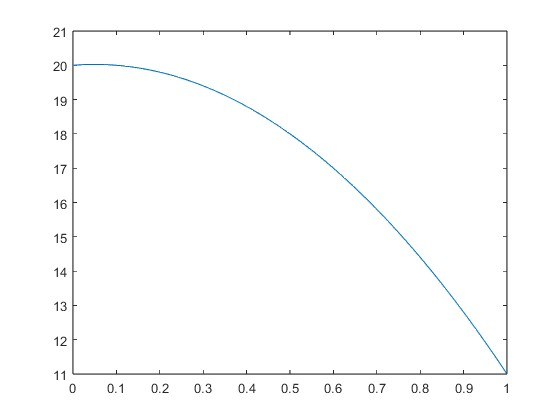
\includegraphics[width=0.8\linewidth]{Graf.jpg}
    \caption{Graf (P, t)}
    \label{fig:enter-label}
\end{figure}
\end{frame}

\begin{frame}{Formula in resitev}
     Formula za trapezno metodo numericnega integriranja: 
    \[\int_a^b f(x)dx = \frac{\Delta x}{2} (f(x_0)+2f(x_1)+2f(x_2)+...+2f(x_{n-1})+f(x_n))\]\
    Resitev:
     \[\int P(t)dt = 17,1665\]\
\end{frame}

\end{document}